\documentclass{article}

\usepackage{amsmath}
\usepackage{amsthm}
\usepackage{mathtools}

\usepackage{tikz}
\usetikzlibrary{calc, intersections}


\title{Algebrauppgift 7 - Dela planet}
\author{Emma Bastås}
\date{November 6, 2022}

\begin{document}

\maketitle

Uppgiften är att visa att om $n$ linjer är ritade på planet så att inga av dem är parallella och så att inga tre linjer skär i en punkt, då delar linjerna planet i $R(n)$ områden där:

\begin{gather*}
  R(n) = \frac{n^{2} + n + 2}{2}\text{.}
\end{gather*}

Innan uppgiften kan lösas måste vi först förstå uppgiften. Linjer, parallella linjer och linjer som skär varandra i punkter är välbekanta koncept vid det här laget, men vad innebär det att \emph{dela planet i områden}? Här saknas tydliga trygga definitioner från kurslitteraturen att falla tillbaka på. I brist på annat får vi tolka uppgiften och ge en egen definition av vad detta innebär. Innan vi betraktar problemet att dela in planet i områden så kan vi istället begränsa oss till atta dela in en cirkel i områden. Betrakta en cirkel i planet:

\begin{center}
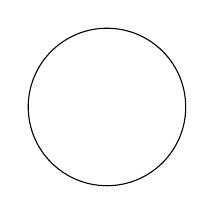
\begin{tikzpicture}
  \draw (0, 0) circle (1cm);
\end{tikzpicture}
\end{center}

Vi säger att denna cirkel delar planer i ett område utanför cirkeln och ett område innanför, just nu intresserar vi oss bara för området inom cirkeln och i kommande resonemang så räknas inte området utanför cirkeln med. Vi säger att vi kan dela in cirkeln i fler områden genom att lägga till linjesegment ett efter ett. Nedan följer en cirkel med tre linjesegment som delar cirkeln i fyra områden.

\begin{center}
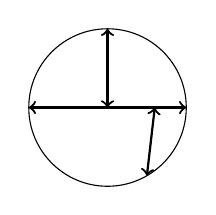
\begin{tikzpicture}[scale=1]
  \draw (0,0) circle (1);

  \coordinate (E) at (0:1);
  \coordinate (N) at (90:1);
  \coordinate (W) at (180:1);
  \coordinate (S) at (270:1);
  \coordinate (O) at (0,0);

  \draw[<->, thick] (W)--(E);
  \draw[<->, thick] (N)--(O);
  \draw[<->, thick] (0.6,0)--(300:1);
\end{tikzpicture}
\end{center}

Vi ställer upp ett antal krav och egenskaper för linjesegmenten:

\begin{itemize}
  \item[(A1)] Flera linjesegment får inte läggas till samtidigt.
  \item[(A2)] Ett linjesegments ändpunkter måste skära cirkeln eller andra linjesegment.
  \item[(A3)] När ett linjesegment läggs till får inga andra punkter än ändpunkterna skära cirkeln eller andra linjesegment.
  \item[(A4)] Ett linjesegments ändpunkter måste vara olika.
  \item[(E)] Relationen mellan antalet linjesegment $LS$ och antalet områden i cirkeln $R$ ges av $R = LS + 1$.
\end{itemize}

Detta är att betraka som en sorts axiom, vi (jag) kan inte med de kunskaper vi besitter ge nåon mer rigorös argumentation till varför dessa krav är rimliga och leder till den fina egenskapen (E), men betrakta nedan exempel på hur (E) slutar gälla om någon av reglerna bryts:

\begin{center}
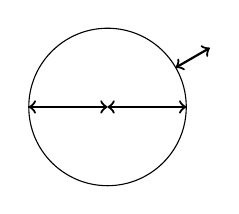
\begin{tikzpicture}[scale=1]
  \draw (0,0) circle (1);

  \coordinate (E) at (0:1);
  \coordinate (N) at (90:1);
  \coordinate (W) at (180:1);
  \coordinate (S) at (270:1);
  \coordinate (O) at (0,0);

  \draw[<->, thick] (W)--(O);
  \draw[<->, thick] (E)--(O);
  \draw[<->, thick] (30:1)--(30:1.5);
\end{tikzpicture}
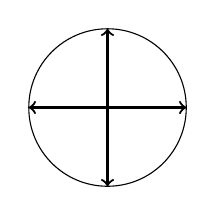
\begin{tikzpicture}[scale=1]
  \draw (0,0) circle (1);

  \coordinate (E) at (0:1);
  \coordinate (N) at (90:1);
  \coordinate (W) at (180:1);
  \coordinate (S) at (270:1);
  \coordinate (O) at (0,0);

  \draw[<->, thick] (N)--(S);
  \draw[<->, thick] (W)--(E);
\end{tikzpicture}
\end{center}


I det första exemplet bryter vi mot (A1) och har lagt till två segment samtidigt, dessa segment uppfyller alla andra krav. Vi har också lagt till ett segment som bryter mot (A2) med en ändpunkt som varken skär cirkeln eller något annat segment. Vår intuition säger oss att cirkeln är delad i två områden men (E) ger att cirkeln är delad i fyra.

I det andra exemplet bryter vi mot (A3) med två linjesegment som skär varandra i andra punkter än ändpunkterna, vår intuition ger fyra områden men (E) ger tre.

Krav (A4) är svår att illustrera, men det inses enkelt att detta kravet är nödvändigt.
\\

Nu kan vi betrakta en cirkel som delas av linjer istället för linjesegment. Vi säger att alla linjer måste skära cirkeln i två punkter (tangenter är alltså inte tillåtna) och att linjer endast får skära varandra i cirkeln. Ett annat sätt att tänka på det är att det istället är cirkeln som alltid är minst så stor som den behöver vara för att inga linjer ska skära varandra utanför cirkeln. Ser vi på det från detta perspektivet så blir det tydligt att detta går att betrakta som att vi delar planet. Oavsett hur linjerna konstrueras så kan cirkeln alltid göras så stor att allt ``spännande'' sker i cirkeln. Nu säger vi att denna värld i vilket vi delar den oändligt stora cirkeln är homomorfisk med den värld där vi delar planet, allt som gäller för den oändliga cirkeln gäller även för planet.

Om vi lägger till en linje så kommer den först att skära cirkeln, efter det skär den eventuellt andra linjer för att sedan skära cirkeln igen och försvinna bort mot oändligheten. Om vi vid varje par av skärningspunkter spänner upp ett linjesegment med ändpunkter i dessa skärningspunkter så kommer dessa linjesegment att följa alla regler (A1-4):

\begin{itemize}
  \item[(A1)] Linjesegment läggs till allt eftersom att linjen skär cirkeln eller andra linjer.
  \item[(A2)] Alla linjesegments ändpunkter ligger på punkter där linjen skär cirkeln eller andra linjer. Eftersom att andra linjer spänner upp linjesegment så kommer en skärningspunkter med en annan linje även att vara en skärningspunkt med ett annat linjesegment.
  \item[(A3)] \emph{TODO, hmnnn....}
  \item[(A4)] Uppenbart sant.
\end{itemize}

Att lägga till en linje med $S$ skärningspunkter är alltså att lägga till $S - 1$ linjesegment i cirkeln.

Med begränsningarna att inga linjer får vara parallella och att tre linjer inte får skära varandra i samma punkt får vi en relation mellan antalet linjer $n$ och antalet linjesegment $LS$. Har vi $n$ linjer och lägger till en ny så kommer denna att skära alla $n$ linjer precis en gång, samt skära cirkeln två gånger vilket ger totalt antal skärningspunkter $S = n + 2$. Antalet nya linjesegment ges av $LS = S - 1$ så vi får då $n + 1$ ny linjesegment. Omskrivet som en rekursiv summa får vi då:

\begin{gather*}
  LS_{n + 1} = LS_{n} + n + 1 \quad n > 0 \\
  LS_{0} = 0\text{.}
\end{gather*}

Vi gissar att denna rekursiva summa är ekvivalent med formeln $(n ^2 + n) / 2$ och bevisar detta med induktion. Basfallet är trivialt, för induktionssteget antar vi att det finns något $n$ så att formeln gäller, då kan $LS_{n + 1}$ skrivas om som:

\begin{align*}
  LS_{n + 1} &= \frac{n^{2} + n}{2} + n + 1 \\
             &= \frac{n^{2} + 3n + 2}{2} \\
  &= \frac{(n + 1)^{2} + (n + 1)}{2}
\end{align*}

och vi har därmed genom induktion visat att $LS = (n^{2} + n) / 2$ för alla $n \geq 0$.

Nu ger oss egenskapen (E) att det totala antalet områden för $n$ linjer är:

\begin{gather*}
  R(n) = LS_{n} + 1 = \frac{n^{2} + n}{2} + 1 = \frac{n^{2} + n + 2}{2}
\end{gather*}

vilket är vad som skulle bevisas.

\centering{$\qed$}

\end{document}
